\documentclass{article}
\usepackage[T1]{fontenc}
\usepackage[utf8]{inputenc}

\usepackage{cmbright}
\usepackage[T1]{fontenc}

\usepackage{multicol}

\usepackage{amsmath}
\usepackage{amsfonts}
\usepackage{amssymb}
\usepackage{tikz}
\usepackage{graphicx}
\graphicspath{  {./images/} }
\setlength{\parindent}{0pt}
\usepackage{changepage}
\usepackage{verbatim}
\usepackage{physics}
\usepackage{derivative}
\usepackage{bm}
\usepackage[colorlinks=true, linkcolor=blue, urlcolor=blue, citecolor=blue, anchorcolor=blue]{hyperref}

\addtolength{\oddsidemargin}{-.25in}
\addtolength{\textwidth}{0.5in}

\makeatletter
\newcommand*\bigcdot{\mathpalette\bigcdot@{.5}}
\newcommand*\bigcdot@[2]{\mathbin{\vcenter{\hbox{\scalebox{#2}{$\m@th#1\bullet$}}}}}
\makeatother

\DeclareMathOperator{\di}{d\!}
\newcommand*\Eval[3]{\left.#1\right\rvert_{#2}^{#3}}

\newcommand{\uvec}[1]{\boldsymbol{\hat{\textbf{#1}}}}
\newcommand{\vr}[1]{\textbf{#1}}

\newcommand{\thus}[0]{\; \; \longrightarrow \; \;}

\newcommand{\lag}{\mathcal{L}}
\newcommand{\ham}{\mathcal{H}}

\title{Merger Rate Calculations Simulations}
\author{Ryan Liu}
\date{Last updated: July 13, 2021}

\begin{document}

\maketitle

\section{Resources Used}

\begin{itemize}
    \item M Fishbach, D Holz, W Farr. \textit{Does the Black Hole Merger Rate Evolve with Redshift?} \url{https://arxiv.org/abs/1805.10270}
    \item LIGO Scientific Collaboration. \textit{Population Properties of Compact Objects from the Second Ligo-Virgo Gravitational Wave Transient Catalog.} \url{https://arxiv.org/abs/2010.14533}
    \item Kremer et al. \textit{Modeling Dense Star Clusters in the Milky Way and Beyond with the CMC Cluster Catalog.} \url{https://arxiv.org/abs/1911.00018}
\end{itemize}



\section{Notes}

Following Fishbach et al., we can describe the mass-redshift distribution of binary black hole (BBH) mergers by 
\begin{equation}
    \frac{dM}{dm_1 dm_2 dz} = M p(m_1, m_2, z)
\end{equation}
where $m_1 \geq m_2$ are the component masses of the black holes, $z$ is the cosmological redshift, $M$ is the total number of mergers, and $p(m_1, m_2, z)$ is the probability that a random BBH merger has parameters $m_1$, $m_2$, and $z$. \\

For simplicity, let us assume that \textbf{the mass and redshift distributions of BBHs are independent of each other}. This may not be true over large redshifts, in particular the full expected detection range of Cosmic Explorer at design sensitivity, but should be a good approximation for the aLIGO and A+ models. Therefore, 
\begin{equation}
    p(m_1, m_2, z) = p(m_1, m_2) p(z)
\end{equation}
By definition, it follows that 
\begin{equation}
    \int_{m_1} \int_{m_2} p(m_1, m_2) dm_1 dm_2 = \int_z p(z) dz = 1
\end{equation}

In this section, we focus on the redshift distribution, and leave the mass distribution to the next section. We consider two possible models for the redshift evolution of BBH merger rates. \textbf{Model A} is a simple power law, and \textbf{Model B} is modeled after the specific star formation rate (SFR):
\begin{gather}
    \textbf{Model A:} \quad p(z | \lambda) \propto \frac{dV_c}{dz} (1+z)^{\lambda-1} \\
    \textbf{Model B:} \quad p(z | \psi) \propto \frac{dV_c}{dz} (1+z)^{-1} \psi(z)
\end{gather}
where $\frac{dV_c}{dz}$ is the differential comoving volume as a function of redshift. In both models, \textbf{the extra factor $(1+z)^{-1}$ takes into account the conversion from source-frame to detector-frame time}. $\psi(z)$ is the SFR: 
\begin{equation}
    \psi(z) \propto \frac{(1+z)^{2.7}}{1 + [(1+z)/2.9]^{5.6}} 
\end{equation}



\section{Calculations}

We parameterize Model A and Model B as follows: 
\begin{gather}
    \textbf{Model A:} \quad Mp(z, c, p) = 4\pi c \Big(\frac{dV_c}{dz}\Big) (1+z)^{p-1} \\
    \textbf{Model B:} \quad Mp(z, c, p, a, b) = 4\pi c \Big(\frac{dV_c}{dz}\Big) \frac{(1+z)^{p-1}}{1 + [(1+z)/a]^b}
\end{gather}
where $c$ is the comoving merger rate in units of $\text{Gpc}^{-3} \text{yr}^{-1}$ at redshift $z=0$ and $p$ is the rate evolution parameter. Clearly, $p=0$ defines a redshift-indepedent merger rate (which is highly unlikely). The additional coefficients $a$ and $b$ are introduced in Model B to allow for variations in the SFR formula. Furthermore, because $\frac{dV_c}{dz}$ is calculated in units of $[L]^3 \text{sr}^{-1}$, both models are multipled by $4\pi$ to convert to units of $[L]^3$. \\

We consider five possible parameterizations of Model A as put forth by Abbott et al., each corresponding to a different mass distribution model: 
\begin{enumerate}
    \setlength{\itemsep}{0pt}
    \item Non-evolving power law + peak: $c = 23.9, p = 0$
    \item Non-evolving truncated: $c = 33, p = 0$
    \item Non-evolving power law + peak, $m_1 \geq 2 M_\odot$: $c = 52, p = 0$
    \item Power law + peak: $c = 19.3, p = 1.3$
    \item Broken power law: $c = 19.3, p = 1.8$
\end{enumerate}
We also consider Model B, using the SFR from Eq. (6). \\

We note that the merger rate density as a function of redshift, which is usually reported in literature, is given by 
\begin{equation}
    \frac{dM}{dV_c dt} (z) = \frac{dM}{dz} \Big[ \frac{dV_c}{dZ} (z) \Big]^{-1} \Big[ \frac{1+z}{T_\text{obs}}\Big]
\end{equation}
where $t$ denotes the source-frame time and $T_\text{obs}$ is the total time of observation of the detector. We see that the $(1+z)$ factor converts from detector-frame to source-frame time. It clearly follows that 
\begin{equation}
    \frac{dM}{dV_c dt} (z) = M p(z) \Big[ \frac{dV_c}{dZ} (z) \Big]^{-1} \Big[ \frac{1+z}{T_\text{obs}}\Big]
\end{equation}
Substituting in Model A for $M p(z)$, it is clear that the simple power law is recovered. 



\section{Results}

We first look at the differential comoving volume and total comoving volume as a function of redshift. As expected, differential comoving volume is highest at redshifts of $\mathcal{O} (1)$. Both lines in Fig. \ref{fig:dist} are in agreement with textbook graphs.  

\begin{figure}[!htb]
    \center{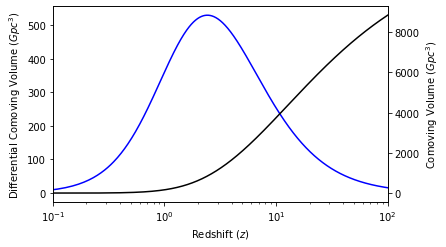
\includegraphics[width=3.5in]{SNR27.png}}
    \caption{\label{fig:dist} Comoving volume (black) and differential comoving volume (blue) as a function of redshift, calculated with AstroPy}
\end{figure}

Plotting hte various merger rate densities as a function of redshift, we see that the models diverge significant for redshifts greater than aLIGO detection range ($z > 1.5$), as expected due to significant uncertainty in the BBH population. However, all models of the total number of mergers within a particular redshift agree to within an order of magnitude of each other, therefore allowing for a rough estimate of the detection results of Cosmic Explorer at design sensitivity. \\

\begin{figure}[!htb]
    \center{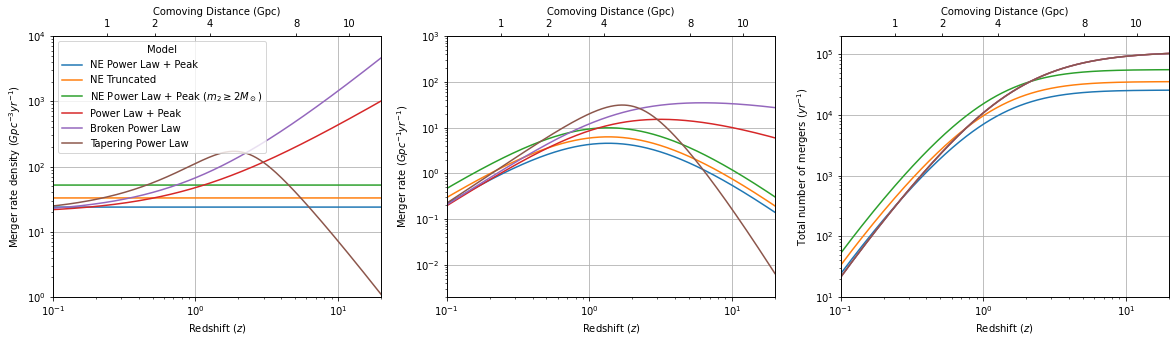
\includegraphics[width=\textwidth]{SNR28.png}}
    \caption{\label{fig:mergerrate} BBH merger rate density (left), merger rate (center), and total number of mergers (right) as a function of redshift based on six possible models of the BBH population as described in Section 3.}
\end{figure}

One possible modification to the power law and non-evolving merger rate models to take care of the inevitable decline in merger rates near Hubble time ($z > 10$) is to apply a smoothing function similar to the one described in the next section for mass distribution, or more simply use a truncated model. However, as seen in the last panel of Fig. \ref{fig:mergerrate}, this will likely not significantly change the predicted number of mergers and detections.





\end{document}












